%%%%%%%%%%%%%%%%%%%%%%%%%%%%%%%%%%%%%%%%%%%%%%%%%%%%%%%%%%%%%%%%%%%%%%%%%%%%%%%%%%%%%%%%%%%%%%%%
%
% CSCI 1430 Final Project Report
%
%%%%%%%%%%%%%%%%%%%%%%%%%%%%%%%%%%%%%%%%%%%%%%%%%%%%%%%%%%%%%%%%%%%%%%%%%%%%%%%%%%%%%%%%%%%%%%%%

\documentclass[10pt,twocolumn,letterpaper]{article}

\usepackage{cvpr}
\usepackage{epsfig}
\usepackage{graphicx}
\usepackage{amsmath}
\usepackage{amssymb}
\usepackage{booktabs}
\usepackage{microtype}

\frenchspacing

\usepackage[pagebackref=true,breaklinks=true,letterpaper=true,colorlinks,bookmarks=false]{hyperref}

\cvprfinalcopy
\def\cvprPaperID{****}
\def\httilde{\mbox{\tt\raisebox{-.5ex}{\symbol{126}}}}
\pagestyle{plain}

\begin{document}

%%%%%%%%% TITLE
\title{CSCI 1430 Final Project Report:\\Watch Me Dance: Webcam-Driven Animation for Drawn Characters}

\author{
    \emph{Team name}: Watch Me Dance\\
    Ian Liu, Chen-En Ma\\
    \emph{TA name:} Kamya Raman
}

\maketitle
\thispagestyle{plain}

%%%%%%%%% ABSTRACT
\begin{abstract}
We extend Meta's Animated Drawings system from an offline, clip-driven animation tool into an interface that can be controlled by uploaded video or a live webcam. The original system analyzes a static drawing, builds a 2D rig and textured mesh, and retargets a prerecorded BVH motion clip to deform the drawing. Our contribution adds two new motion sources: an RGB-video-to-BVH adapter and a real-time webcam controller based on MediaPipe pose landmarks. The offline path estimates the body landmarks required by Animated Drawings, repairs unreliable tracks with temporal interpolation and rule-based smoothing, and converts the result into a BVH motion sequence that can drive the existing renderer. The live path skips file generation and maps a causal MediaPipe stream directly into character pose updates. We also evaluated a conditional rectified-flow landmark corrector on synthetic BVH-derived corruptions, but leave it disabled in the final system because it does not improve the primary L1 and PCK metrics. The complete prototype supports uploaded drawings, bundled characters, uploaded or recorded motion clips, live camera control, quality reporting, and fallback behavior when pose estimates are unreliable.
\end{abstract}

%%%%%%%%% BODY TEXT
\section{Introduction}

Traditional character animation separates drawing, rigging, motion capture, retargeting, and rendering into specialist workflows. Meta's \emph{Animated Drawings} project lowers one part of this barrier: a user can upload a humanoid drawing and animate it with a prerecorded BVH motion clip~\cite{Smith2023AnimatedDrawings}. However, the released pipeline still depends on existing motion clips. A child or casual creator cannot simply stand in front of a webcam, wave, and see the drawing wave back.

Our project asks whether a simple RGB camera can become the control signal for this drawing animation pipeline. This is difficult for three reasons. First, monocular human pose estimates are noisy, especially under occlusion, cropping, and fast motion. Second, MediaPipe, BVH files, and the Animated Drawings rig use different coordinate systems, joint names, depth conventions, and skeleton topologies. Third, the live version must be causal: it cannot rely on future frames to clean up the current estimate.

We address these issues by treating motion estimation as an adapter around the existing renderer. The drawing analysis, mesh construction, and rendering stages remain largely intact. We add a motion layer that maps RGB video or webcam frames into the joint orientations expected by Animated Drawings. In offline mode, this layer converts a recorded video into reusable character motion. In live mode, it estimates pose frame by frame and drives the character directly.

\begin{figure*}[t]
    \centering
    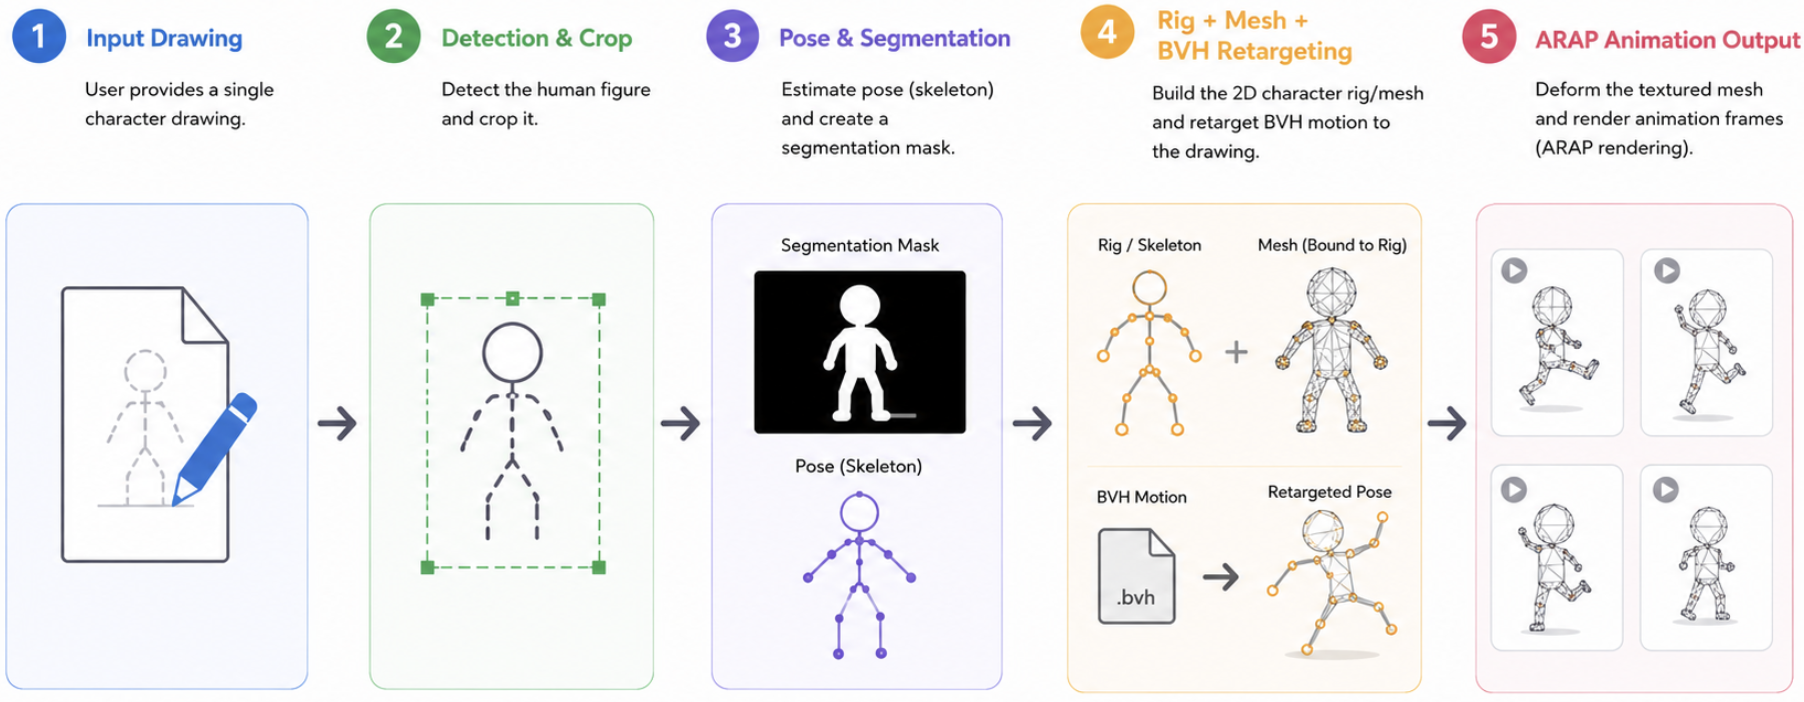
\includegraphics[width=\textwidth,height=0.25\textheight,keepaspectratio]{figure1.png}
    \caption{End-to-end Animated Drawings asset and rendering workflow. A static character image is localized, segmented, converted into a 2D rig and mesh, driven by a BVH motion sequence, deformed, and composited into output animation frames.}
    \label{fig:original-workflow}
\end{figure*}

\section{Related Work}

\paragraph{Animated drawings.}
The base repository implements Smith et al.'s method for animating children's drawings of human figures~\cite{Smith2023AnimatedDrawings,FacebookAnimatedDrawingsRepo}. Their system detects the drawn figure, segments it, predicts a 2D skeleton, constructs a textured deformable mesh, and retargets human motion to the drawing. We keep this core design and extend the motion input stage.

\paragraph{Human pose estimation.}
We initially considered OpenPose, VideoPose3D, and MocapNET. OpenPose introduced part affinity fields for real-time multi-person 2D pose association~\cite{Cao2017OpenPose}. VideoPose3D shows how temporal convolutions can lift 2D keypoints into temporally consistent 3D pose~\cite{Pavllo2019VideoPose3D}. MocapNET is especially relevant because it predicts BVH-compatible pose from 2D joints~\cite{Qammaz2019MocapNET}. For the implemented prototype, we chose MediaPipe Pose because it is lightweight, easy to run locally, and designed for real-time single-person tracking~\cite{Lugaresi2019MediaPipe,Bazarevsky2020BlazePose,MediaPipePoseDocs}. MediaPipe produces 33 normalized body landmarks; our converter uses the 13 landmarks required by the existing retarget configuration.

\paragraph{Motion representation and deformation.}
BVH is a common skeletal motion format containing a joint hierarchy and per-frame channels~\cite{BlenderBVHDocs,CMUMocap}. Animated Drawings deforms a 2D textured mesh using an as-rigid-as-possible formulation inspired by Igarashi and Igarashi~\cite{Igarashi2009ARAP}. Our work therefore sits at the boundary between camera pose estimation and graphics retargeting.

\section{Method}

\subsection{Original Animated Drawings Pipeline}

The original pipeline has two separable stages. The first turns a drawing image into character assets: a foreground texture, a mask, a visual skeleton overlay, and a 2D rig. The system detects the drawn humanoid, crops the main figure, segments it from the background, and predicts a 16-joint skeleton. These assets define the drawing that the renderer later deforms.

The second stage retargets a BVH motion clip to this 2D character. The retargeter normalizes the source skeleton, chooses projection planes for body-part groups, and converts projected BVH bones into 2D character bone orientations. Conceptually, each controlled character bone is oriented by comparing the projected source bone direction against the character's upright reference axis.

The resulting 2D rig drives a textured mesh through ARAP deformation, which preserves local shape while satisfying the skeleton handle constraints. The renderer then draws the deformed texture with optional depth ordering from the retargeted joints. Our project leaves this asset and rendering pipeline intact and changes only how motion reaches it.

\subsection{MediaPipe Video-to-BVH Pipeline}

Our offline extension starts from an RGB video and estimates MediaPipe Pose landmarks for each frame. Each landmark contains normalized image coordinates, relative depth, and a visibility score. Although MediaPipe provides 33 landmarks, our converter keeps the body points required by the drawing retargeter: nose, shoulders, elbows, wrists, hips, knees, and ankles.

Low-confidence landmarks are repaired before BVH conversion. For each coordinate, frames below a visibility threshold are linearly interpolated from nearby visible frames when possible, then smoothed over a short temporal window. The postprocessor also checks for likely left-right swaps, sudden jumps in the hip center, and foot-contact jitter. When the hip center moves implausibly between adjacent frames, later frames are shifted back toward the previous root trajectory. These operations produce a quality report covering a variety of metrics such as detection coverage and foot stabilizations.

The BVH converter constructs a compact skeleton rooted at the hips. For each frame, it recenters the landmarks at the image-space hip center, scales them into BVH units, and flattens them into a frontal plane by treating horizontal image displacement as side-to-side motion and vertical image displacement as up-down body motion. This deliberate flattening matches the primarily 2D drawing system. Bone directions in this coordinate frame are converted into parent-relative joint rotations and written as a standard BVH motion sequence. The output can then be used anywhere Animated Drawings expects a motion clip.

\begin{figure*}[t]
    \centering
    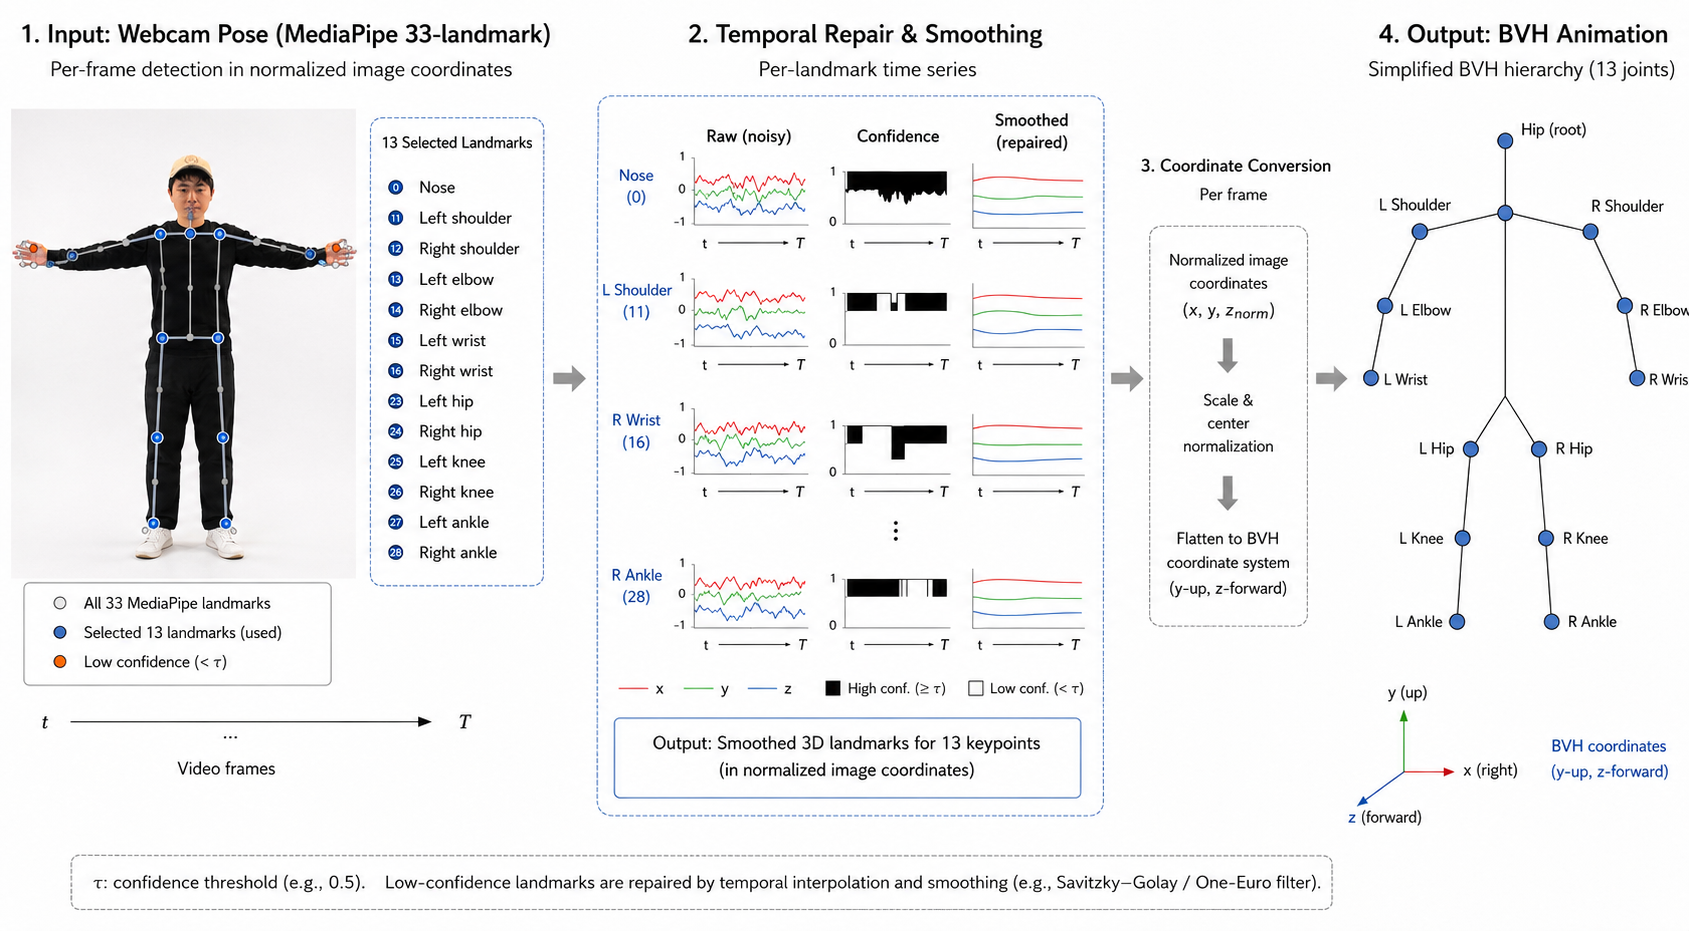
\includegraphics[width=\linewidth,height=0.34\textheight,keepaspectratio]{figure2.png}
    \caption{Offline MediaPipe-to-BVH motion adapter used in our extension. RGB video landmarks are filtered by visibility, temporally repaired and smoothed, mapped into a flattened hip-centered coordinate frame, and packaged as reusable character motion.}
    \label{fig:mediapipe-bvh}
\end{figure*}

\subsection{Live Webcam Retargeting}

The live webcam mode cannot wait for a full video or write a BVH file at each frame. Instead, it replaces the file-based motion clip with a streaming controller that returns the current joint orientations, depth ordering, and root position directly to the renderer.

For each webcam frame, MediaPipe estimates the current pose. A causal smoother keeps the last good value for invisible landmarks and applies exponential moving average smoothing:
\begin{equation}
\hat{p}_{t,j}=
\begin{cases}
\beta p_{t,j}+(1-\beta)\hat{p}_{t-1,j}, & s_{t,j}\ge \tau,\\
\hat{p}_{t-1,j}, & s_{t,j}<\tau.
\end{cases}
\label{eq:ema}
\end{equation}
The live point conversion uses $(x,1-y,z)$ so that image coordinates align with the character's 2D frame. The same projected-bone orientation logic is then applied frame by frame. The character can either stay anchored in place or move with the user's hip displacement after an initial reference pose.

\subsection{Landmark-Flow Ablation}

We also explored, but did not enable by default, a learned temporal postprocessor for unreliable landmarks. The model is a conditional rectified-flow network over 31-frame landmark windows, following the idea of learning a velocity field between paired source and target samples~\cite{Liu2022RectifiedFlow}. Training data is generated from BVH files by forward kinematics, random orthographic projection, and synthetic corruption. Each clean clip is $y\in\mathbb{R}^{T\times J\times2}$ with $T=31$ and $J=13$. The condition is
\begin{equation}
c=\left[x_{\mathrm{corrupt}},\,s,\,m\right],
\end{equation}
where $m_{t,j}=1$ marks corrupted or low-confidence landmarks.

For $t_f\sim U(0,1)$, the rectified-flow state is a straight-line interpolation between corrupt and clean coordinates:
\begin{equation}
y_{t_f}=(1-t_f)x_{\mathrm{corrupt}}+t_f y.
\end{equation}
The target velocity is $u=y-x_{\mathrm{corrupt}}$. A temporal convolutional model $f_\theta(y_{t_f},c,t_f)$ is trained with masked SmoothL1 reconstruction plus a small temporal velocity-smoothness penalty:
\begin{equation}
\begin{aligned}
\mathcal{L}(\theta)=
&\frac{\sum_{t,j}m_{t,j}\rho\left(f_\theta(y_{t_f},c,t_f)_{t,j}-u_{t,j}\right)}
{\sum_{t,j}m_{t,j}+\epsilon}\\
&+\lambda_s\frac{1}{T-1}\sum_{t=1}^{T-1}
\left\|f_{\theta,t+1}-f_{\theta,t}\right\|_1 .
\end{aligned}
\label{eq:flow-loss}
\end{equation}
At inference, Euler integration starts from the corrupt landmarks and applies $K=8$ velocity steps:
\begin{equation}
\hat{y}^{k+1}=\hat{y}^{k}+\frac{1}{K}f_\theta(\hat{y}^{k},c,k/K).
\end{equation}
In the final system, the active repair path remains the non-learned temporal baseline. The flow corrector is retained as an ablation because its test results did not justify replacing the simpler method.

\section{Results}

\subsection{Implemented System}

The completed prototype turns Animated Drawings into a camera- and video-driven animation system. In offline use, a short video is converted into pose tracks, a visual pose overlay, a BVH motion clip, and quality metrics. In the web interface, users can choose bundled characters, upload their own drawings, upload existing motion clips, or generate new motion from video. In live use, the system estimates MediaPipe pose frame by frame and renders the driven drawing beside the camera view.

Table~\ref{tab:system} summarizes the main capabilities of the implemented system. The goal of these checks is not only to confirm that files can be produced, but also to show that the motion adapter, live controller, upload flow, and repair logic work as coherent user-facing features.

\begin{table}[t]
\begin{center}
\scriptsize
\resizebox{\linewidth}{!}{%
\begin{tabular}{lcc}
\toprule
Capability & Output & Status \\
\midrule
Pose extraction & landmark tracks & works \\
Video motion export & BVH clip & works \\
Render setup & motion metadata & works \\
Quality reporting & diagnostics & works \\
Live control & webcam motion & works \\
Web upload flow & interactive UI & works \\
Temporal repair & cleaner tracks & works \\
Flow ablation & metrics & \shortstack{comparable L1/PCK,\\ improved RMSE} \\
\bottomrule
\end{tabular}
}
\end{center}
\caption{Implemented system capabilities. The flow ablation result is reported in detail in Table~\ref{tab:flow-results}.}
\label{tab:system}
\end{table}

\IfFileExists{figure3.png}{
\begin{figure}[t]
    \centering
    \includegraphics[width=\linewidth,height=0.24\textheight,keepaspectratio]{figure3.png}
    \caption{Qualitative retargeting examples from the implemented system. Each example compares the source pose signal, the intermediate skeleton or BVH representation, and the resulting 2D animated drawing to show how webcam or uploaded-video motion is transferred to the character.}
    \label{fig:qualitative}
\end{figure}
}{}

\subsection{Landmark Correction Evaluation}

The learned landmark-flow corrector was trained for 100 epochs with hidden size 128, dropout 0.1, AdamW, 31-frame windows, and 13 landmarks. On the synthetic BVH-derived test split, it did not meet our acceptance target of improving masked L1 by 10\% over the repair baseline. The final system therefore uses the non-learned repair path. Table~\ref{tab:flow-results} reports the flow model's standalone error profile: its RMSE is reasonable on harder long-span and whole-limb corruptions, but its L1 and PCK are not strong enough to justify enabling it by default.

\begin{table}[t]
\begin{center}
\scriptsize
\begin{tabular}{lccc}
\toprule
Subset & L1 $\downarrow$ & RMSE $\downarrow$ & PCK $\uparrow$ \\
\midrule
Overall & 0.0155 & 0.0148 & 0.852 \\
Long spans & 0.0187 & 0.0176 & 0.764 \\
Whole limb & 0.0181 & 0.0170 & 0.784 \\
\bottomrule
\end{tabular}
\end{center}
\caption{Landmark-flow ablation metrics. Lower L1/RMSE is better; higher PCK@0.02 is better. These results characterize the learned repair experiment; the final system keeps the non-learned repair path because the learned model did not meet the acceptance target.}
\label{tab:flow-results}
\end{table}

\subsection{Technical Discussion}

One main technical lesson is that format compatibility is not the same as motion quality. A BVH file may load successfully while still producing awkward animation if its coordinate frame, joint semantics, or temporal smoothing do not match the drawing rig. Our 2D-to-BVH conversion works best for frontal gestures such as waving, arm raises, and simple stepping, but it cannot recover true out-of-plane rotation from monocular landmarks. MediaPipe's $z$ values are useful as relative cues, but we do not treat them as metric 3D reconstruction.

The live controller is often visually more stable for immediate interaction because it avoids quantizing motion into a simplified BVH hierarchy. The tradeoff is reusability: a saved BVH can be replayed, inspected, and rendered with different characters, while live retargeting is an ephemeral stream.

The learned corrector also clarified the strength of simple baselines. Temporal interpolation and rule-based smoothing are difficult to beat when corruptions are short and the underlying motion is smooth. The flow model's lower RMSE on long and whole-limb corruptions suggests that learned repair could still help with large failures, but its weaker PCK means it often misses the tight 0.02 normalized-coordinate threshold. A practical next version could train a residual model or apply learned repair only when confidence diagnostics predict that the baseline will fail.

\subsection{Social Impact}

This project can make animation more accessible to students, hobbyists, and children by turning body movement into an immediate creative input. That democratization is valuable, but it is not impact-free. Easier animation tools may increase the volume of low-cost animated content and could reduce demand for some pose-based prototyping work. We view the system as a sketching and educational tool rather than a replacement for professional animation judgment, but deployment should avoid implying that automated webcam retargeting substitutes artistic labor.

Because the interface can use live or recorded video, privacy is the highest-risk issue, especially for younger users. Webcam-driven tools should make local processing clear, avoid unnecessary retention of video, and communicate when camera data leaves the machine. If the system is used by minors, it should require parent or guardian consent, avoid storing identifiable clips by default, and never use a user's video or pose traces for further training without explicit opt-in. Even pose landmarks can be sensitive behavioral data, so exported overlays, pose JSON, and BVH files should be treated as user data rather than harmless metadata.

There is also an accessibility and bias tradeoff. The current interaction assumes a webcam, sufficient physical space, and the ability to make large, camera-visible body movements. People with limited mobility, atypical movement patterns, different body proportions, loose clothing, low lighting, or lower-quality cameras may receive worse pose estimates and less recognizable animations. A more inclusive version would support prerecorded motion clips, manual pose editing, seated or upper-body modes, and examples that show a wider range of bodies and movement styles.

Finally, although our prototype is not a conversational companion, self-created animated characters can still invite attachment, particularly for children. The tool should be framed as a creative animation workspace, not as a synthetic friend or emotionally responsive partner. If future versions add sharing, character generation, or dialogue, they should include age-appropriate guardrails and avoid design patterns that encourage dependency or parasocial substitution.

\section{Conclusion}

We built a working webcam- and video-driven extension to Animated Drawings. The final system preserves the original drawing analysis and ARAP rendering pipeline while adding MediaPipe motion estimation, temporal repair, BVH conversion, live retargeting, and a web interface. The main contribution is a practical bridge from camera pose to drawn-character motion. The landmark-flow model remains useful as an experiment, but the deployed system keeps the simpler repair path until learned correction consistently improves the primary metrics.

{\small
\bibliographystyle{plain}
\bibliography{ProjectFinal_ProjectReportTemplate}
}

\clearpage
\section*{Appendix}

\IfFileExists{appendix_realtime_test.png}{
\subsection*{Realtime Test Screenshot}

\begin{figure}[h]
\centering
\includegraphics[width=\linewidth]{appendix_realtime_test.png}
\caption{Realtime webcam retargeting test. The left panel shows MediaPipe pose tracking over the live camera frame, while the right panel shows the selected Animated Drawings character driven by the estimated pose.}
\label{fig:appendix-realtime-test}
\end{figure}
}{}

\subsection*{Team contributions}

\noindent\textbf{Ian Liu.}
Integrated externally generated motion into the Animated Drawings renderer, worked on retargeting compatibility between MediaPipe-style motion and drawing rigs, configured rendering workflows, and implemented or tested the interactive webcam and web application pieces that connect drawings, motion sources, and rendered output.

\medskip
\noindent\textbf{Chen-En Ma.}
Investigated RGB-video-to-motion pipelines, tested 2D pose estimation options including OpenPose and MediaPipe, implemented the MediaPipe pose extraction and video-to-BVH conversion path, and trained/evaluated the landmark-flow correction model for low-confidence landmark repair.

\end{document}
